\section{Results}\label{sec:results}
% All numbers are final. Sources: thesis/PAPER_NUMBERS.md (scratchpad), which cites each result file
% and CSV line. "Legacy" = the two legacy checkpoints (optimizer foot point = fpopt_legacy; calcaneus
% origin = sept_legacy), trained on the stored labels with the inverted sign. "Corrected" = qc_s1-s3
% (optimizer foot point, init seeds 1-3) and qc_origin (calcaneus origin, seed 1); physical sign.
% "3-seed ensemble" = averaged predictions (mean F_y and M_x of qc_s1-s3), NOT the mean of per-seed
% metrics; it beats every single seed on held-out MAE and r (audit_test_seeds/summary.csv).
% Lencioni = the data folders named "tiziana".
%   D1: gc/knee_jr/stored_check.csv (status 'stored check': 139 GC trials; 65 with vasti > 1 BW frames,
%       stored_below_vas_r_frac median 1.000, min 0.814; stored_r_F_max_bw median 0.809 over 139;
%       so_vas_r_max_bw max 8.37); 95 % of 8,037 walking trials (gc/pilot_AB_sojr/README.md "OpenSim
%       label sources"); stance-peak |F_y| of the four-lab training pool (labels_qc/per_trial.csv,
%       split training, walking, carter/moore/tiziana/falisse: 7,991 trials, 82 people, 7,772 with both
%       stance peaks, medians 1.266 -> 6.971; all six labs incl. Fregly/Han would give 1.26 -> 6.86).
%   D2: labels_qc/mx_sign/README.md sections 2-5 (population scan: up to 300 walking trials per
%       lab); legacy vs stored-label moment r -0.54 / -0.35 (audit_gc/qc_keep/label_agreement.csv
%       lines 26, 12); Carter lateral moment: SO+JR r through the 30-40 % bin, stored through 40-50 %
%       (mx_sign section 4); 80.6 % = facts X02.
%   D3: qc_final.md fix:so-diagnosis and verify:so-diagnosis; 30/30 covered windows, median ratio 1.90
%       (recomputed from audit_gc/frames.csv.gz + halves.csv: cover >= 0.9, max |F_y| SO+JR vs max
%       meas_tot per window; the pilot set labels_qc/fregly_vs_measured.csv gave 27/27, 1.91).
%       P003 t05 COP: labels_qc/carter_P003_t05_cop_vs_foot.csv (one right stance, 0.764-1.364 s,
%       cop_x 0.8518-0.8576 m). Quality-checked frames (training-consistent mask carry): audit_gc/
%       qc_keep/summary.csv lines 39, 30, 47 (SO+JR medial bias +0.43 JW, +0.61 DM, +0.26 SC; SC 732 of
%       1,244 frames, total bias +0.86). SC's 24 re-solved frames: labels_qc/
%       resolve_random_stance_stats.csv. kutzner2010 = instrumented TKA patients.
%   Table I: labels_qc/rules.csv lines 338 (12,152 s of stance), 351 (mask_any_so 67.1 %), 352.
%   Table II: audit_gc/summary.csv; inverted row audit_gc_legacy_pipeline_sign/summary.csv;
%       corrected = 3-seed ensemble, qc_keep/summary.csv lines 16, 7, 24; seed ranges
%       qc_keep/seed_spread.csv.
%   In vivo text: audit_gc/README.md; legacy early-peak miss 1.2-1.6 BW (qc_keep/peaks.csv);
%       JW SO+JR late bias 2.9247 -> 2.92; scored windows per knee and half 3-6 (qc_keep/peaks.csv
%       n_windows: DM 3/3, JW 5/4, SC 4/6).
%   D4: facts X01 (offsets), M10 (rates), X02 (80 ms, 80.6 % of training frames). S3 legacy in
%       vivo: audit_gc_legacy_native vs audit_gc (JW 1.132 -> 1.103 BW).
%   Table III: results/fmedial_eval/audit_test_qc (summary.csv walking/ALL/stance, sweep.csv phi 0.5
%       d 45; trials.csv subset stance for the foot-point medians: fpopt vs sept legacy 0.0188, qc_s1
%       vs qc_origin 0.0191, qc_s1 vs qc_s3 0.0234, 605 trials) and audit_test_seeds (ensemble:
%       MAE 0.413, r 0.785, peak -0.851, recall 0.872, precision 0.842); person-mean stance MAE
%       0.483 / 0.626 / 0.518, legacy 1.259 (audit_test_qc/README.md); sep23/summary.csv and pairs.csv
%       (S2 pelvis conversion, S4); twente/audit_twente/seed_disagreement_table.csv (seg-static,
%       U_gyro: ens13 0.380, qc_s2 0.266, 3-seed ens 0.333; median over 9 people of the per-person
%       mean over speeds).
%   S2: converter = pipeline/label_trajectory_csv.py line 81 (written for this study, not by [4]).
%   S4: results/thesis/sep23 (README: pinned COP at x = 0.131-0.134 m in the calcn frame, which alone
%       fails the fixed-COP rule; pelvis conversion 12.9 deg, foot 11.01 cm as written; the effect of the
%       mis-mapping on the labels is untested; legacy in the pipeline sign with converted angles: S1
%       means 0.79 / 1.04, peaks 1.66 / 2.04; spread.csv 0.73 / 1.02 BW; summary.csv; pairs.csv
%       qc_origin - qc_s1 +0.30 BW, 77 % outside the band).
%   Corrected baseline: qc_keep/summary.csv (kept frames: JW r 0.41 vs 0.87, SC 0.47 vs 0.74),
%       qc_keep/stance_shape.csv, qc_keep/peaks.csv lines 48-50 (SC late +0.31 / +1.55 / +1.60);
%       seed 2 recall 0.982, precision 0.807 (audit_test_qc/sweep.csv).
%   Wearable: results/thesis/pn3_sim (headline.csv, seed_detail.csv, backdating.csv, README);
%       twente/audit_twente (angles_table.csv lines 289, 737: median over 9 people; seed_disagreement_
%       table.csv lines 131, 147; headline.csv contact_agree_gyro_r). Per-frame cost re-timed
%       2026-11-10 with qc_s1 (driver run() loop on the moore_s10 1-deg take, one thread, estimator +
%       two contact detectors + surrogate, 749 frames after 60 warm-up: mean 2.36-2.42 ms in three
%       repeats; scratchpad apply/time_driver.py). The older 4.5 ms (facts A3-36) is superseded.

% ---------------------------------------------------------------------------------------------
\begin{table}[t]
\caption{SO+JR Label Quality}
\label{tab:qc}
\centering\footnotesize
\setlength{\tabcolsep}{3pt}
\begin{tabular}{@{}lcc@{}}
\toprule
Lab & Peak $|F_y|$ (BW) & Fixed COP (\%)\\
\midrule
Carter   & 2.16 $\to$ 10.79 & 95.0 (94.8)\\
Moore    & 1.20 $\to$ 6.49  & $\le$0.4\\
Lencioni & 0.98 $\to$ 6.39  & 51.9 (87.7)\\
Falisse  & 1.00 $\to$ 5.12  & 30.8 (43.5)\\
\midrule
Rule & Defect & Stance time (\%)\\
\midrule
COP $<$0.2~m/s (trial)                & fixed COP & 42.8\\
Knee-crossing muscle saturated        & SO        & 30.3\\
$\ge$3 leg muscles saturated          & SO        & 19.4\\
Leg reserve $>$0.1~N$\cdot$m/kg       & SO        & 11.9\\
Ankle co-activation $>$0.5            & SO        & 17.6\\
Activation jump $>$0.5 per 10~ms      & SO        & 23.3\\
Pelvis residual $>$5\%                & dynamics  & 43.4\\
Any SO or dynamics rule               & --        & 67.1\\
$|F_y| > 5$~BW                        & magnitude & 29.2\\
\midrule
Kept for training                     &           & 25.4\\
Dropped by the legacy filters         &           & 95.0\\
\bottomrule
\end{tabular}\\[2pt]
\parbox{\columnwidth}{\scriptsize Top: median right-knee stance peak of $|F_y|$ in training
walking (stored $\to$ SO+JR); share of trials (of stance time) with a fixed COP. Bottom: share of
training-pool right-knee stance time (7,991 trials, 12,152~s of stance) that each rule flags. The
5~BW flag is reported, not applied.}
\end{table}

\subsection{Labels Without Muscle Forces (D1)}\label{sec:res-d1}
In the 65 of 139 Grand Challenge trials with frames where the SO vasti force exceeded 1~BW, the
stored knee force was below the vasti force alone in a median of all such frames (at least 81\%
per trial), although a label that applied the SO forces would include that pull. The stored force
peaked at a median 0.81~BW, while the vasti alone reached up to 8.4~BW. The same held in 95\% of
the 8,037 walking trials with such frames. Relabelling with the SO forces raised the median stance
peak of $|F_y|$ in the training pool from 1.27 to 6.97~BW (7,772 trials with a right stance, 82
people; Table~\ref{tab:qc}). The stored labels under-read the implants' medial and total force,
though their medial force correlates with the measured one (Table~\ref{tab:invivo}).

\subsection{Inverted Moment Sign (D2)}\label{sec:res-d2}
All three checks agree: the medial-positive moment is $-M_x$ at the right knee and $+M_x$ at the
left ($s = -1$ and $+1$), the opposite of the convention ($s = +1$ at the right knee) in the
pipeline's training and inference code. Only this sign returns the medial force from synthetic
contact loads; in every lab's model the medial knee-muscle points of the right leg lie at $z =
-0.018$ to $-0.024$~m and the lateral ones at $+0.027$ to $+0.035$~m; and in Kaneda et al.'s
results, $r(M_x, F_{\mathrm{med}} - F_{\mathrm{lat}})$ is $-0.99$ (JW), $-0.91$ (DM) and $+0.99$
(SC).

With the physical sign, every OpenSim moment rises with the implant's medial-minus-lateral force
($r = 0.29$--0.48 over label sources and knees). The legacy surrogates looked plausible against the
implants only under their inverted sign; under the physical sign, their medial force
anti-correlates with the implant in all three subjects (Table~\ref{tab:invivo}). The sign is not
the only cause: on JW and DM their moment also anti-correlates with the stored-label moment they
were trained on ($r = -0.54$, $-0.35$), whatever the sign, and Carter's labels (80.6\% of legacy
training frames, stored and SO+JR alike) carry a non-physiological lateral moment over roughly the
first 40\% of stance (longer in the stored labels) that the surrogates reproduce. The inverted sign
made this artefact look like a normal early adduction peak.

\subsection{SO+JR Label Defects (D3)}\label{sec:res-d3}
SO+JR labels are implausibly high. The median per-step stance peak of moving-COP trials is
6.18~BW for Carter (60 trials, 4 people) and 6.58~BW for Moore (1,677 trials), 2.4 to 2.5 times
the in vivo walking peak of about 2.6~BW in knee-replacement patients~\cite{kutzner2010}. On the
implants, SO+JR total force exceeds the measured force in all 30 covered stance windows (median
ratio 1.90).

\textit{Fixed COP.} The fixed point is already present in the AddBiomechanics GRF. In Carter trial
P003~t05, the right COP stays within 6~mm ($x = 0.852$--$0.858$~m) through the stance in which the
knee load peaks at 9.99~BW, 0.108~s after foot strike, with a GRF of only 1.21~BW at 36$^\circ$ of
knee flexion.

\textit{Unconverged SO.} At one Carter frame, the stored SO cost was 2.8 times the optimum;
re-solving lowered the summed knee-crossing muscle force from 7.2 to 3.4~BW. Of
149 random moving-COP stance frames, 31.5\% were non-optimal; their median $|F_y|$
was 3.64~BW against 2.18~BW at optimal frames, and re-solving would bring it to about 2.15~BW.

\textit{Causes.} Of the 40 hand-picked peaks above 4~BW, 36 trace to the three defects (fixed COP
7, unconverged SO 22, dynamic inconsistency 7). The rules keep a quarter of pool stance time
(Table~\ref{tab:qc}); a 5~BW cap would remove only another 2.5\% of it. The defects do not explain
all of the excess: on SC, where none of 24 re-solved stance frames was non-optimal, SO+JR still
over-reads total force by 0.86~BW on the 732 stance frames (59\%) that pass the rules, and on such
frames it over-reads medial force in all three knees (by 0.26--0.61~BW).

% ---------------------------------------------------------------------------------------------
\begin{table}[t]
\caption{Medial Force Against the Implants}
\label{tab:invivo}
\centering\footnotesize
\setlength{\tabcolsep}{2.6pt}
\begin{tabular}{@{}lcccccc@{}}
\toprule
 & \multicolumn{2}{c}{JW (right)} & \multicolumn{2}{c}{DM (right)} & \multicolumn{2}{c}{SC (left)}\\
Source & bias & $r$ & bias & $r$ & bias & $r$\\
\midrule
Stored labels           & $-0.87$ & 0.82 & $-0.63$ & 0.49 & -- & --\\
\quad total force       & $-0.80$ & 0.53 & $-1.37$ & $-0.21$ & -- & --\\
SO+JR labels            & $+0.62$ & 0.64 & $+0.60$ & 0.45 & $+0.50$ & 0.56\\
\quad total force       & $+1.25$ & 0.72 & $+0.90$ & 0.41 & $+1.18$ & 0.68\\
Kaneda et al.\ SO+JR$^a$ & -- & -- & -- & -- & $-0.03$ & 0.86\\
Legacy, optimizer pt.   & $-1.07$ & $-0.54$ & $-0.74$ & $-0.13$ & $-1.24$ & $-0.25$\\
Legacy, calcaneus       & $-1.05$ & $-0.51$ & $-0.75$ & $-0.13$ & $-1.24$ & $-0.29$\\
Legacy, inverted$^b$    & $-0.22$ & 0.70 & $-0.42$ & 0.35 & $-0.86$ & 0.44\\
Corrected$^c$           & $+0.53$ & 0.35 & $+0.84$ & 0.22 & $+0.17$ & 0.30\\
\midrule
Frames (segments)       & \multicolumn{2}{c}{889 (27)} & \multicolumn{2}{c}{878 (24)} & \multicolumn{2}{c}{1,244 (43)}\\
\bottomrule
\end{tabular}\\[2pt]
\parbox{\columnwidth}{\scriptsize Physical moment sign; bias = predicted minus measured (BW);
Pearson $r$ over instrumented-limb stance frames. DM is conditional on its timing. $^a$On 1,021
SC frames in its windows (ours there: $+0.46$, 0.64). $^b$Optimizer-point model, inverted
sign. $^c$Ensemble of seeds 1--3 (averaged predictions); seed ranges: bias $+0.47$ to
$+0.58$, $+0.71$ to $+0.96$, $+0.15$ to $+0.19$; $r$ 0.32--0.39, 0.14--0.32, 0.26--0.36 (JW, DM,
SC).}
\end{table}

% ---------------------------------------------------------------------------------------------
\begin{figure}[t]
\centering
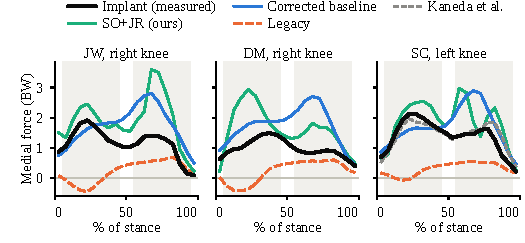
\includegraphics[width=\columnwidth]{figures/fig2_invivo.pdf}
\caption{Medial force against the implants: means of instrumented-limb stance frames in 5\%
bins (physical sign; SC only in Kaneda et al.'s windows). Corrected: 3-seed ensemble.
Legacy: optimizer-point model. Shading: peak windows.}
\label{fig:invivo}
\end{figure}

\subsection{Input Construction (D4)}\label{sec:res-d4}
The legacy builder sampled the position windows on an even grid over the whole IK segment,
including the 0.3-s SO buffers, while joint angles, flags and labels sat on the JR frames. On an
8-s Carter trial this shifted positions against labels by $-0.300$ to $+0.304$~s (mean
absolute 0.151~s), and on a Moore and a Lencioni trial by up to 0.18 and 0.075~s. The builder also
kept each lab's native rate (100--250~Hz), so a 20-frame window spanned 80~ms on Carter trials
(80.6\% of training frames) but 200~ms on Moore trials and in deployment. The test features shared
the warp, so held-out scores could not reveal it.

\subsection{In Vivo Medial Force}\label{sec:res-invivo}
SO+JR over-reads medial force (MAE 0.64--0.66~BW; Table~\ref{tab:invivo}, Fig.~\ref{fig:invivo}).
It has the double hump, but its early peaks are too high by 0.58--1.35~BW and its late peaks by
1.64 (SC) and 2.92~BW (JW) (3--6 windows per knee and half). Its medial share of axial force
(0.54--0.61) matches the implant's (0.48--0.71), so the excess is in the total force. On the same SC frames, Kaneda et al.'s released SO+JR reaches an MAE of 0.28~BW,
against 0.61~BW for ours. Stored labels and legacy surrogates miss the early peak by 1.14--1.51
and 1.2--1.6~BW.

% ---------------------------------------------------------------------------------------------
\begin{table}[t]
\caption{Held-Out Accuracy and Sensitivity}
\label{tab:sens}
\centering\footnotesize
\setlength{\tabcolsep}{3pt}
\begin{tabular}{@{}lcc@{}}
\toprule
Quantity & Legacy & Corrected\\
\midrule
Held-out $\Fmed$ MAE (BW)                 & 1.26 & 0.43--0.44\\
Held-out $\Fmed$ $r$                      & 0.46 & 0.70--0.77\\
Stance-peak error (BW)                    & $-2.02$ & $-0.86$ to $-0.81$\\
Limit recall / precision                  & 0.003 / 0.64 & 0.70--0.98 / 0.81--0.91\\
S1: recall, $\phi$--$d$ grid              & 0.001--0.005 & 0.49--0.99\\
S2: foot-point swap$^a$ (BW)              & 0.019 & 0.019\\
S2: pelvis angles$^b$ (BW)                & $+0.11$ & $-0.05$ to $-0.01$\\
S3: training $\to$ aligned$^c$ (BW)       & 1.13 $\to$ 1.10 & --\\
S4: reference, stance-1 mean (BW)         & 0.26 & 1.80--2.45\\
S4: reference, stance $>$1.4~BW (\%)      & 0 & 100\\
Xsens: IMU vs optical$^d$ (BW)            & -- & 0.38\\
\bottomrule
\end{tabular}\\[2pt]
\parbox{\columnwidth}{\scriptsize Physical sign throughout. Held-out rows: right-knee walking
stance frames of the test split with quality-checked SO+JR labels (33,915 frames of five people,
93\% from one Moore person); aligned inputs. Legacy: optimizer-point model. Corrected: range over
seeds 1--3; their ensemble (averaged predictions) beats each seed: MAE 0.41, $r$ 0.78, peak error
$-0.85$, recall 0.87, precision 0.84. $^a$Median absolute change of trial MAE, 605 trials (seed 1
vs.\ 3: 0.023); the legacy pair also differ in training run. $^b$Mean change of the reference
stance reading when pelvis angles are converted. $^c$In vivo MAE, JW. $^d$$\Fmed$ MAE, all
frames, median over 9 people; ensemble of seeds 1 and 3 (damped seed 2: 0.27; all three: 0.33);
static calibration, gyro contact.}
\end{table}

\subsection{Sensitivity}\label{sec:res-sens}
\textit{S1.} The constants trade off against label bias. Against the implants, SO+JR fits best
at the grid corner ($\phi = 0.4$, $d = 50$~mm) in all three subjects (MAE 0.40--0.52~BW, against
0.64--0.66~BW at the nominal values), still over-reading by 0.14--0.29~BW; the stored labels fit
best at $\phi = 0.6$. The same 1.4~BW limit therefore marks different loads for different label
sources. On the test split, the share of limit crossings that the seeds catch varies widely over
the grid (Table~\ref{tab:sens}).

\textit{S2.} The foot point changes held-out accuracy no more than swapping seeds does
(Table~\ref{tab:sens}). The converter we used to prepare the optimizer's reference motion for
OpenSim copies its pelvis angles, which rotate about other axes, into OpenSim's pelvis coordinates
(errors up to 12.9$^\circ$ in stance). Converting them barely moves the corrected readings of that
motion, but there the calcaneus-origin run reads 0.30~BW above seed~1, outside the seed range in
77\% of stance frames.

\textit{S3.} Scored in vivo, aligning the legacy inputs changes their error by at most 0.03~BW
(Table~\ref{tab:sens}).

% ---------------------------------------------------------------------------------------------
\begin{figure}[t]
\centering
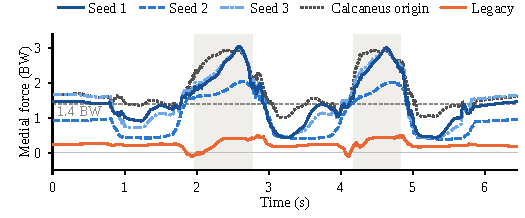
\includegraphics[width=\columnwidth]{figures/fig_sep23_seeds.pdf}
\caption{$\Fmed$ on the locked-knee reference motion of the optimizer of \Chong{}~\citeChong{},
which has no usable labels (same inputs for every model, pelvis angles converted; physical sign).
Legacy: optimizer-point model. Shading: right single stance. Dashed: 1.4~BW limit.}
\label{fig:refmotion}
\end{figure}

\textit{S4.} The SO+JR labels of the reference motion are unusable. Its COP stays at the
optimizer's mid-foot contact point through every single stance, which alone makes the fixed-COP rule
remove every right-knee frame; the copied pelvis angles (S2) also place the scaled model's foot
11.0~cm on average from the applied COP, an effect on the labels we did not test. We therefore
compare the models with each other (Fig.~\ref{fig:refmotion}). Read with the physical sign, every corrected run exceeds 1.4~BW in every
frame of both right single stances, and both legacy models stay below it (Table~\ref{tab:sens});
with their (inverted) training sign, the legacy models read stance-1 means of 0.79--1.04 and
peaks of 1.66--2.04~BW. Corrected and legacy models thus fall on opposite sides
of the limit, and without labels nothing on this motion shows which side is right. The seeds agree
on the verdict but not on the load: their per-frame range averages 0.73 and reaches 1.02~BW,
mostly due to seed~2.

\subsection{Corrected Baseline}\label{sec:res-corrected}
On held-out walking, the corrected seeds track SO+JR far more closely than the legacy model, which
learned the stored labels (Table~\ref{tab:sens}); the labels exceed 1.4~BW in 70\% of these
stance frames, and the seeds catch most of these crossings, the legacy model almost none. In vivo
(Table~\ref{tab:invivo}, Fig.~\ref{fig:invivo}), the baseline correlates positively in all three
knees, where the legacy models anti-correlate. But it inherits the over-read of its labels, has
one late hump at 60--70\% of stance instead of two, and tracks the implants less well than its
labels, also on quality-checked frames (JW $r$ 0.41 vs.\ 0.87, SC 0.47 vs.\ 0.74). Seeds with
equal pooled held-out error (person means 0.48, 0.63 and 0.52~BW) do not tie elsewhere: seed~2
flags the most crossings (recall 0.98, but precision 0.81) and is closest to the implants in every
knee (SC late peak $+0.31$ vs.\ $+1.55$ and $+1.60$~BW), yet reads the reference motion lowest.

\subsection{Wearable Path}\label{sec:res-wearable}
On the simulated suit (two held-out trials, 1$^\circ$ noise), the worst joint-angle
root-mean-square error (RMSE) was 2.1$^\circ$ and 1.8$^\circ$. Contact detection, not orientation
noise, drove the deviation of $\Fmed$ from the same surrogate fed with mocap: in stance 0.16 and
0.22~BW with the gyro detector against 0.07 and 0.06~BW with force-plate contact (seed~1; gyro
seed means 0.12 and 0.18). Back-dating cut the deviation from 0.24 to 0.16~BW on one trial
but only from 0.23 to 0.22~BW on the
other, where the detector re-triggered in 3 of 11 left swings, and it left the error against
quality-checked labels unchanged (0.43~BW, seed~1). A full driver frame
costs about 2.4~ms on one CPU thread, well within the 16.7-ms suit period.

On the 54 Xsens trials of 9 people, the UKF's right knee angle differed from optical IK by a median
per-person RMSE of 5.0$^\circ$ (mostly a $-3.5^\circ$ offset), against 2.2$^\circ$ for the vendor's
angles. $\Fmed$ on IMU input differed from that on optical input (Table~\ref{tab:sens})
mostly through contact: with treadmill contact flags the difference was
0.14~BW. The gyro detector agreed with the treadmill in only 0.64--0.73 of frames below 1.25~m/s,
against 0.84--0.86 at 1.25--1.50~m/s, where the difference fell to about 0.2~BW; in a pilot, the
swing foot turned at only 150--320$^\circ$/s at 0.25--0.75~m/s, below the 400$^\circ$/s release
threshold.
